\chapter{Kernzerfälle und -spaltung}
\begin{compactitem}
\item Verschiedene Zerfallsmoden
\item (Historisch) erster Zugang zur schwachen WW
\item Kernspaltung $\lt$ Kettenreaktionen
\end{compactitem}
\section{\texorpdfstring{$\alpha$}{}-Zerfall von Kernen}
Emission eines $\alpha$-Teilchens $= \ ^4_2\text{He}_2$-Kern (He-Kern doppelt magisch)
\begin{align}
\boxed{
^A_Z X_N \ra ^{A-4}_{Z-2} Y_{N-2} + \alpha
}
\end{align}
\begin{figure}[!ht]
\centering
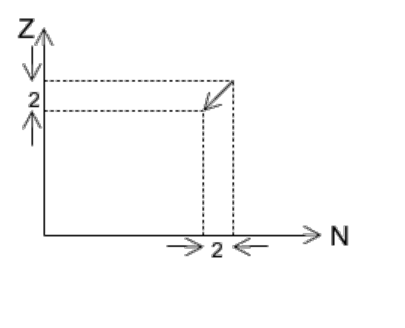
\includegraphics[width=.4\textwidth]{imgs/ep5-fig-5-1.pdf}
\caption{$\alpha$-Zerfall in der Nuklidebene \label{fig:5.1}}
\end{figure}
\begin{itemize}
\item Energiebilanz:
\begin{align}
\boxed{
M(A,Z) = M(A-4, Z-2) + M_\alpha + Q
}
\end{align}
$Q\ =\ Q$-Wert
\item[$\lt$] Zerfall ist möglich, wenn $Q>0$
\item[$\lt$] Wegen $M_\alpha \overset{\text{i.d.R.}}{\ll} M(A-4, Z-2)$ ist $Q\approx T_\alpha$
\item[$\lt$] Bei p, n-Emission ist $Q$ um $E_B(\alpha)$ kleiner
\begin{compactitem}
\item[$\lt$] kommt nur sehr selten vor
\end{compactitem}
\item[$\lt$] 2-Körper-Endzustand
\begin{itemize}
\item[$\Ra$] für gegebenen Zerfall hat $T_\alpha$ immer den gleichen Wert
\item[$\Ra$] \glqq Linienspektrum\grqq
\end{itemize}
Deutung/Interpretation:\\
Im Kern formiert sich $\alpha$-Teilchen, das Kern durch Tunnelvorgang verlassen kann

\begin{minipage}[c]{.45\textwidth}
\captionsetup{type=figure}
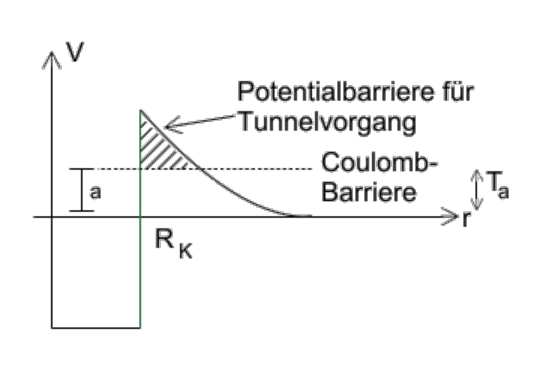
\includegraphics[width=\textwidth]{imgs/ep5-fig-5-2.pdf}
\captionof{figure}{Potentialtopf mit Coulomb- und Tunnelbarriere \label{fig:5.2}}
\end{minipage}
\begin{minipage}[c]{.45\textwidth}
\captionsetup{type=figure}
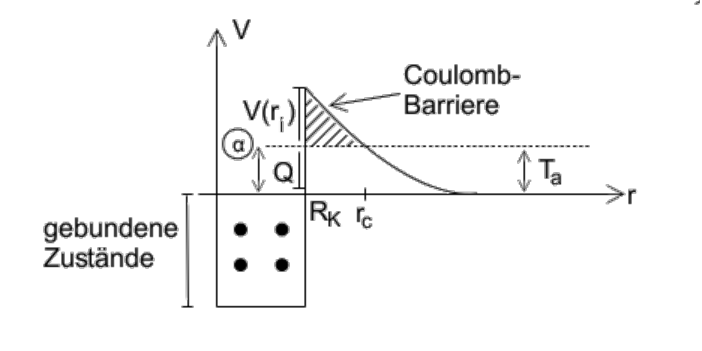
\includegraphics[width=\textwidth]{imgs/ep5-fig-5-3.pdf}
\captionof{figure}{Tunnelbarriere für ein $\alpha$-Teilchen aus dem Kernpotential \label{fig:5.3}}
\end{minipage}

\item \textbf{Tunnelwahrscheinlichkeit} für Barriere mit Breite $\Pa r$ und Höhe $v(r)$
\begin{align}
\boxed{
\Pa p_i = \exp \left( - \frac{2}{\hbar} \sqrt{2 m_\alpha (v(r) -Q)}\ \Pa r \right)
}
\end{align}
Damit ergibt sich die gesamte Tunnelwahrscheinlichkeit zu 
\begin{align}
P \ = \prod_i \Pa p_i = \exp \left( - \frac{2}{\hbar} \int_{R_k}^{r_C} \sqrt{ 2 m_\alpha \left(v(r) -Q\right)} \Pa r \right) = \exp \left(-2G\right)\\
\boxed{G = \frac{1}{\hbar} \int_{R_k}^{r_C} \sqrt{2 m_\alpha \left(v(r) -Q\right)}\Pa r}\\
\sim \ \text{Gamov-Faktor}\nonumber
\end{align}
Annahme (starke Näherung):
\begin{align}
\begin{split}
V(r) = V_C(r), \ r>R_k\\
\Ra V(r) = \frac{2 \left( Z-2\right)\alpha}{r} = \frac{r_C}{r} \underbrace{V\left(r_C\right)}_Q = \frac{r_C}{r} \underbrace{Q}_{T_\alpha}
\end{split}
\end{align}
Hier ohne Rechnung:
\begin{align}
\begin{split}
G = \sqrt{\frac{2 m_\alpha}{T_\alpha}}\cdot 2 \cdot \left(Z-2\right) \cdot \alpha \cdot f\left(\frac{r_C}{R_k}\right)\\
G \approx \frac{2 \pi \alpha \left(Z-2\right)}{\beta_\alpha}
\end{split}
\end{align}
\item Zerfallskonstante:
\begin{align}
\boxed{ \lambda = \omega \cdot \frac{\beta_\alpha}{2 R_k} \cdot e^{-2G}}
\end{align}
\begin{compactitem}
\item[mit] $\omega$: Wskt., dass ein $\alpha$ im Kern gebildet wird
\item[] $\frac{\beta_\alpha}{2R_k}$: Rate der Tunnelversuche
\item[] $e^{-2G}$: Tunnelwahrscheinlichkeit
\end{compactitem}
\begin{align}
\ln \lambda = - \ln \tau = - a_1 \frac{Z-2}{\sqrt{T_\alpha}} + a_2 \dots\\
\sim \ \text{Geiger-Nutall-Regel}\nonumber
\end{align}
\item \tb{Anmerkungen:}
\begin{itemize}
\item $V_C$, $T_\alpha$ sind sehr unterschiedlich für $\alpha$-Strahlung:
\begin{itemize}
\item[$\Ra$] Großer Wertebereich für $e^{-2G}$
\item[$\Ra$] Lebensdauer $\boxed{\tau = 10^{-8}\,\mr{s} \dots 10^{17}\,\mr{a}}$
\end{itemize}
\item Die Rechnung hängt von der genaueren Form von $V(r)$ ab
\item Nicht berücksichtigt: Bahndrehimpuls (Zentrifugalbarriere)
\end{itemize}
\end{itemize}

\section{Beta-Zerfall von Kernen\label{sec:5.2}}
\begin{itemize}
\item[$\ra$] $\beta \ \hat{=}\ e^-\text{ oder }e^+$
\item[$\ra$] 3 Varianten
\item \tb{$\beta^-$-Zerfall}
\begin{align}
\boxed{ \underbrace{^A_ZX_N}_{M\left(A,Z\right)} \longrightarrow \underbrace{^A_{Z+1} X^\prime_{N-1} + e^-}_{M\left(A,Z+1\right)} + \bar{\nu}_e }
\end{align}
Energetisch möglich, wenn:
\begin{align}
\boxed{ M\left(A,Z\right) > M\left(A,Z+1\right) + m_\nu } \qquad m_\nu \approx 0
\end{align}
\begin{itemize}
\item Zerfall durch schwache Wechselwirkung
\begin{figure}[!ht]
    \centering
    \begin{tikzpicture}
        \begin{feynman}
            \vertex (a1) {$u$};
            \vertex[right=6cm of a1] (a2) {$u$};
            \vertex[right=3cm of a1] (a3);
            \vertex[below=2em of a1] (b1) {$d$};
            \vertex[below=2em of a2] (b2) {$d$};
            \vertex[right=3cm of a1] (b3);
            \vertex[below=2em of b1] (d1) {$u$};
            \vertex[right=3cm of d1] (d2);
            \vertex[below=2em of b2] (d3) {$d$};
            %% Equivalent way to obtain (d):
            % \vertex at ($(b2)!0.5!(b3) + (0, -0.5cm)$) (d);
            \vertex[below=of d3] (c1) {$e^-$};
            \vertex[below=2em of c1] (c3) {$\bar \nu_e$};
            \vertex at ($(c1)!0.5!(c3) - (2cm, 0)$) (c2);
            \diagram* {
            (b1) -- [fermion] (b2),
            (d1) -- [fermion] (d2) -- (d2) -- [fermion] (d3),
            (c3) -- [fermion] (c2) -- [fermion] (c1),
            (d2) -- [scalar, edge label=$W^-$] (c2),
            (a1) -- [fermion] (a2),
            };
            \draw [decoration={brace}, decorate] (d1.south west) -- (a1.north west)
            node [pos=0.5, left] {$n$};
            \draw [decoration={brace}, decorate] (a2.north east) -- (d3.south east)
            node [pos=0.5, right] {$p$};
        \end{feynman}
    \end{tikzpicture}
    \caption{Feynmandiagramm des $\beta^-$-Zerfalls \label{fig:5.4}}
\end{figure}
\item 3-Körper-Zerfall\\
$\Ra$ kontinuierliches Spektrum, kontinuierliche Energieverteilung auf Elektron und Neutrino (später genauer)
\item Möglichkeit, z.B. für freie Neutronen
\begin{align}
n \ra p + e^- + \bar{\nu}_e \qquad \tau = 880\,\mr{s}
\end{align}
\end{itemize}

\item \tb{$\beta^+$-Zerfall:}
\begin{align}
\boxed{ \underbrace{^A_ZX_N}_{M\left(A,Z\right)} \longrightarrow \underbrace{^A_{Z-1} X^\prime_{N+1} + e^+}_{M\left(A,Z-1\right)+2 m_e} + \nu_e }
\end{align}
$2m_e$ durch entstehendes $e^+$ und übriges $e^-$\\
Energetisch möglich:
\begin{align}
\boxed{ M\left(A,Z\right) > M\left(A,Z-1\right) + 2m_e + m_\nu }
\end{align}
\begin{itemize}
\item Feynman-Diagramm (schwacher Zerfall)
\begin{figure}[!ht]
    \centering
    \begin{tikzpicture}
        \begin{feynman}
            \vertex (a1) {$u$};
            \vertex[right=6cm of a1] (a2) {$u$};
            \vertex[right=3cm of a1] (a3);
            \vertex[below=2em of a1] (b1) {$d$};
            \vertex[below=2em of a2] (b2) {$d$};
            \vertex[right=3cm of a1] (b3);
            \vertex[below=2em of b1] (d1) {$u$};
            \vertex[right=3cm of d1] (d2);
            \vertex[below=2em of b2] (d3) {$d$};
            %% Equivalent way to obtain (d):
            % \vertex at ($(b2)!0.5!(b3) + (0, -0.5cm)$) (d);
            \vertex[below=of d3] (c1) {$\nu_e$};
            \vertex[below=2em of c1] (c3) {$e^+$};
            \vertex at ($(c1)!0.5!(c3) - (2cm, 0)$) (c2);
            \diagram* {
            (b1) -- [fermion] (b2),
            (d1) -- [fermion] (d2) -- (d2) -- [fermion] (d3),
            (c3) -- [fermion] (c2) -- [fermion] (c1),
            (d2) -- [scalar, edge label=$W^+$] (c2),
            (a1) -- [fermion] (a2),
            };
            \draw [decoration={brace}, decorate] (d1.south west) -- (a1.north west)
            node [pos=0.5, left] {$p$};
            \draw [decoration={brace}, decorate] (a2.north east) -- (d3.south east)
            node [pos=0.5, right] {$n$};
        \end{feynman}
    \end{tikzpicture}
    \caption{Feynmandiagramm des $\beta^+$-Zerfalls \label{fig:5.5}}
\end{figure}
\item Dieser Zerfall ist nicht möglich für freie Protonen, da $m_p < m_n$. Für gebundene Protonen dagegen wird die Massendifferenz durch die Bindungsenergie kompensiert.
\end{itemize}

\item \tb{Elektron-Einfang} (vgl. Abb.\ref{fig:5.6})\\
Ein $e^-$ aus der Atomhülle wird vom Kern eingefangen.\\
Typisch: \glqq K-Einfang\grqq, Einfang aus der K-Schale
\begin{align}
^A_ZX_N \ra ^A_{Z-1} X_{N+1}^{\prime\,(*)} + \nu_e
\end{align}
Energetisch möglich, wenn
\begin{align}
\boxed{ M\left(A,Z\right) \geq M\left(A,Z-1\right) + \mc{E}}
\end{align}
\begin{compactitem}
\item[mit] $\mc{E}$: Anregungsenergie der Atomhülle des Tochterkerns
\end{compactitem}
\begin{itemize}
\item Auffüllen des Loches in der Elektronenhülle erzeugt charakteristische Röntgenstrahlung

\begin{figure}[!ht]
\centering
    \begin{tikzpicture}
    \begin{feynman}
    \vertex (a1);
    \vertex[below = 5em of a1] (b1) {$u$};
    \vertex[below = 2em of b1] (c1) {$u$};
    \vertex[below = 2em of c1] (d1) {$d$};
    \vertex[right = 6cm of a1] (a2);
    \vertex[below = 5em of a2] (b2) {$d$};
    \vertex[below = 2em of b2] (c2) {$u$};
    \vertex[below = 2em of c2] (d2) {$d$};
    \vertex[right = 3cm of b1] (b3);
    \vertex[above = 4em of b3] (a3);
    
    \diagram*{
    (a1) -- [fermion, edge label = $e^-$] (a3) -- [fermion, edge label = $\nu_e$] (a2),
    (b1) -- [fermion] (b3) -- [fermion] (b2),
    (c1) -- [fermion] (c2),
    (d1) -- [fermion] (d2),
    (a3) -- [scalar, edge label = $W^-$] (b3),
    };
    \draw [decoration={brace}, decorate] (d1.south west) -- (b1.north west)
    node [pos=0.5, left] {$p$};
    \draw [decoration={brace}, decorate] (b2.north east) -- (d2.south east)
    node [pos=0.5, right] {$n$};
    \end{feynman}
    \end{tikzpicture}
\caption{Feynmandiagramm des Elektroneneinfangs \label{fig:5.6}}
\end{figure}
\item Energetisch günstiger als $\beta^+$-Zerfall wegen der fehlenden $2m_e$-Terme
\end{itemize}
\item \tb{Betazerfall und Massenparabeln}\\
Tröpfchenmodell (festes $A$):
\begin{align}
\boxed{ M\left(A,Z\right) \ \hat{=} \ \text{Parabel } \left(Z^2\right)}
\end{align}

\begin{figure}[!ht]
\centering
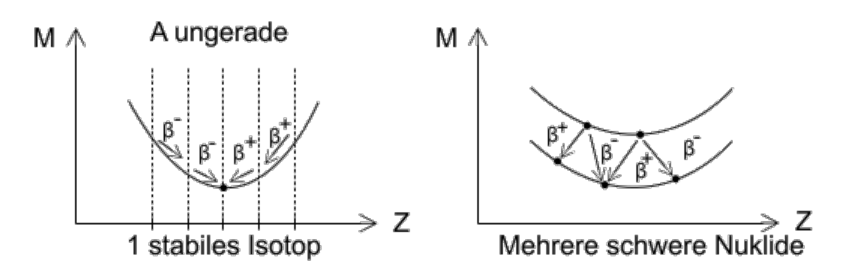
\includegraphics[width=.75\textwidth]{imgs/ep5-fig-5-7.pdf}
\caption{Massenparabel für verschiedene Ausgangsbedingungen\label{fig:5.7}}
\end{figure}

\item \tb{Betazerfall in der Nuklid-Ebene}

\begin{figure}[!ht]
\centering
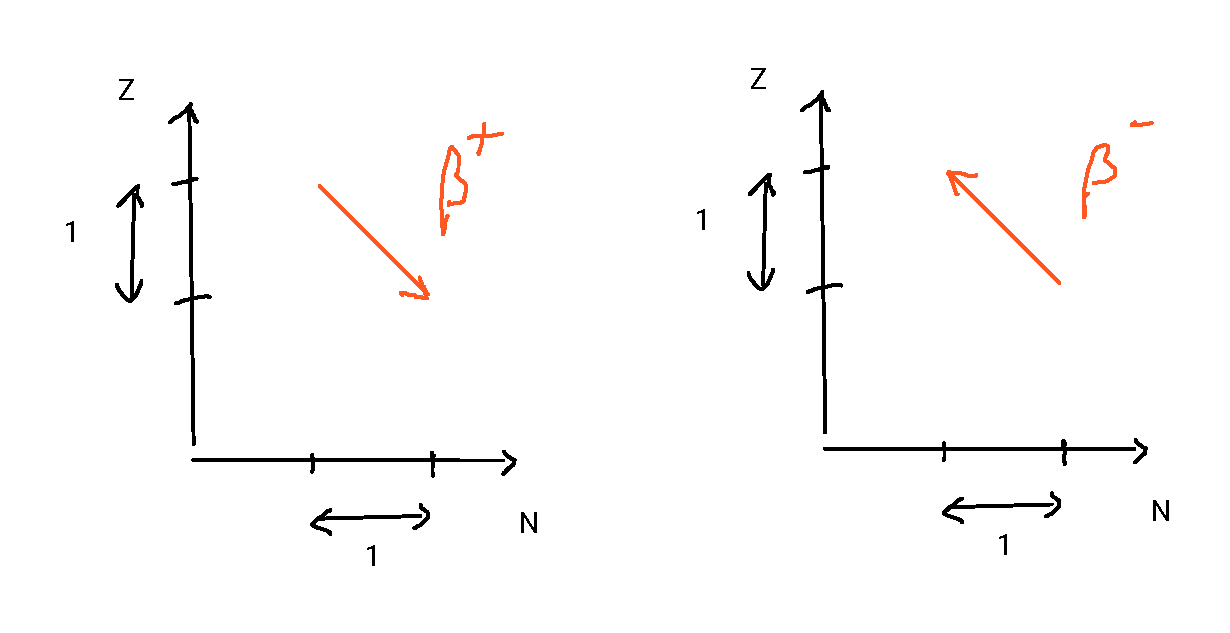
\includegraphics[width=.5\textwidth]{imgs/ep5-fig-5-8.pdf}
\caption{Umwandlung eines Kerns unter $\beta^+$-Zerfall (links) und $\beta^-$-Zerfall (rechts) in der Nuklid-Ebene \label{fig:5.8}}
\end{figure}
\item \tb{$e^{\pm}$-Energiespektrum}\\
Beobachtet: $e^{\pm}$ haben kontinuierliches Energiespektrum
\begin{align*}
0 \leq E_\mr{kin}^e \leq \lno E_\mr{kin}^e\rabs_\mr{max} \approx Q
\end{align*}
\begin{figure}[!ht]
\centering
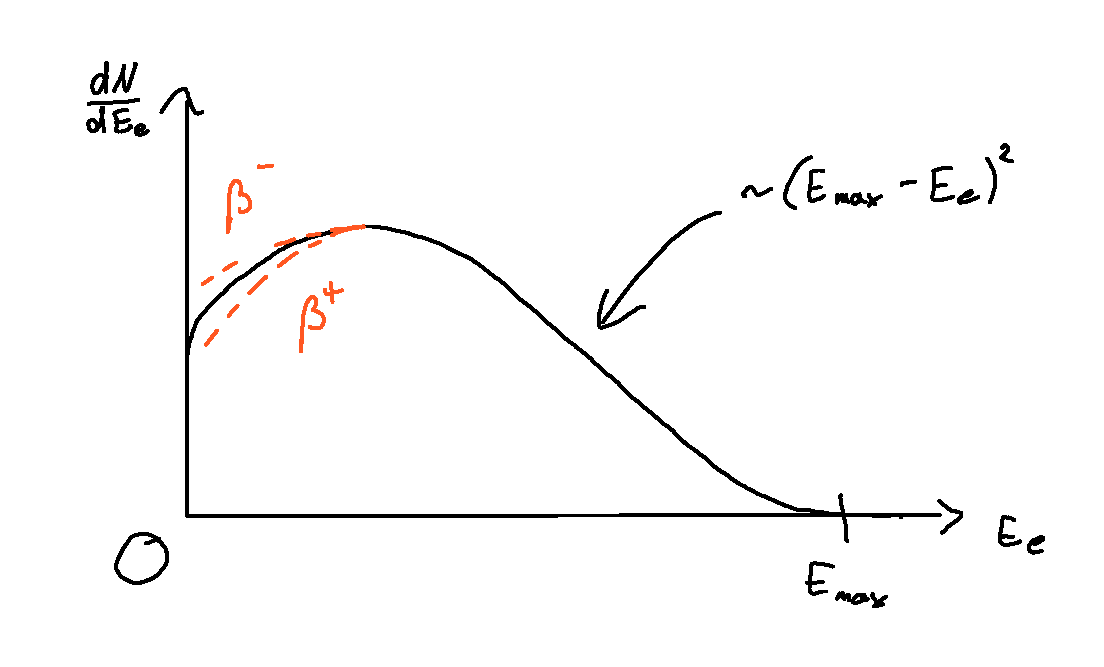
\includegraphics[width=.5\textwidth]{imgs/ep5-fig-5-9.pdf}
\caption{Energiespektrumsgrafik der $e$-Energie\label{fig:5.9}}
\end{figure}
$\leadsto$ 1930: Verletzung von $E$- und $p$-Erhaltung oder neues Teilchen!
\begin{compactitem}
\item[$\Ra$] Pauli postuliert Neutrino
\item[$\Ra$] Nachgewiesen 1956
\end{compactitem}
\item \tb{$\beta$-Zerfall und Neutrinomasse}\\
Wenn $m_\nu > 0$ $\Ra$ $\lno E_\mr{kin}^e\rabs_\mr{max} \approx Q-m_\nu$\\
$\Ra$ Änderung des E-Spektrums bei $\lno E^e_\mr{kin}\rabs_\mr{max}$
\begin{figure}[!ht]
\centering
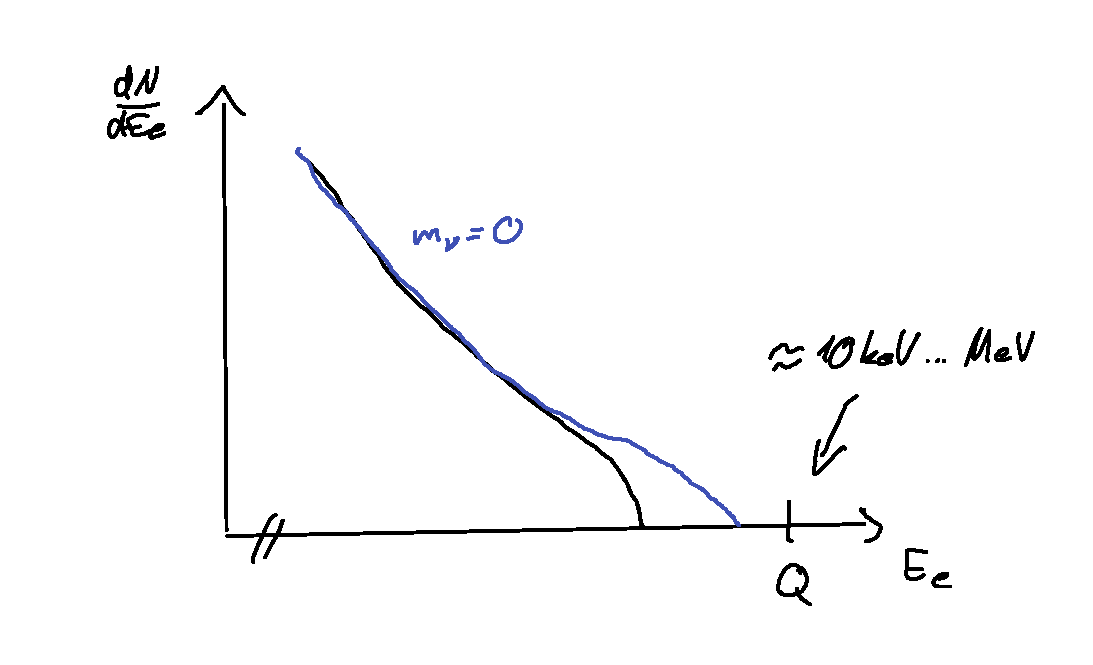
\includegraphics[width=.5\textwidth]{imgs/ep5-fig-5-10.pdf}
\caption{Korrektur (schwarz), wenn Neutrinos massenbehaftet sind\label{fig:5.10}}
\end{figure}

Messung erfordert:
\begin{compactitem}
\item Höchste Messgenauigkeit
\item kleiner $Q$-Wert
\end{compactitem}
Derzeit:
\begin{align}
\boxed{m_\nu < 1.1\,\mr{eV} \text{ mit } 90\,\% C.L.}
\end{align}
aus Tritium-Zerfall
\begin{align*}
^3_1\mr H \underset{Q=18.6\,\mr{keV}}{\ra}\, ^3_2 \mr{He} + e^- + \bar{\nu}_e
\end{align*}
(zukünftig: KATRIN in Karlsruhe: $\sim 0.2\,\mr{eV}$)
\end{itemize}

\section{Doppelbeta-Zerfall}
Falls mehrere stabile Isobare ($\ra$ gg-Kerne):\\
Zerfall durch \glqq 2 simultane Betazerfälle\grqq{} .
\begin{figure}[!ht]
\centering
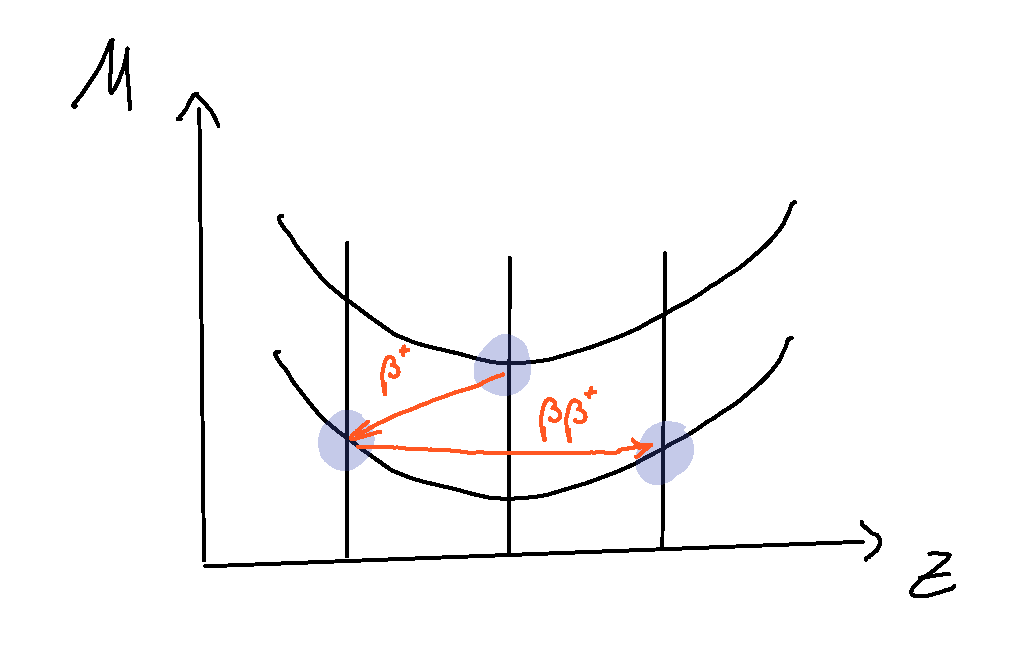
\includegraphics[width=.5\textwidth]{imgs/ep5-fig-5-11.pdf}
\caption{Doppelbeta-Zerfall aufgetragen mit der Masse über die Ordnungszahl\label{fig:5.11}}
\end{figure}
\begin{align}
 ^A_Z X_N \ra ^A_{Z\pm 2} Y_{N\pm 2} + 2e^\pm + 2 \bar{\nu}_e (\text{oder } + 2\nu_e)
\end{align}
\begin{itemize}
\item[$\lt$] Prozess höherer Ordnung (extrem unterdrückt, aber möglich)\\
\begin{figure}[!ht]
    \centering
    \begin{tikzpicture}
        \begin{feynman}
            \vertex (a1) {$u$};
            \vertex[right=6cm of a1] (a2) {$u$};
            \vertex[right=3cm of a1] (a3);
            \vertex[below=2em of a1] (b1) {$d$};
            \vertex[below=2em of a2] (b2) {$d$};
            \vertex[right=3cm of a1] (b3);
            \vertex[below=2em of b1] (d1) {$u$};
            \vertex[right=3cm of d1] (d2);
            \vertex[below=2em of b2] (d3) {$d$};
            \vertex[below=2em of d3] (c1) {$\nu_e$};
            \vertex[below=2em of c1] (c3) {$e^+$};
            \vertex at ($(c1)!0.5!(c3) - (2cm, 0)$) (c2);
            
            \vertex[below=10em of d1] (f1) {$u$};
            \vertex[right=6cm of f1] (f2) {$d$};
            \vertex[right=3cm of f1] (f3);
            \vertex[below=2em of f1] (g1) {$d$};
            \vertex[below=2em of f2] (g2) {$d$};
            \vertex[right=3cm of f1] (g3);
            \vertex[below=2em of g1] (h1) {$u$};
            \vertex[right=3cm of h1] (h2);
            \vertex[below=2em of g2] (h3) {$u$};
            \vertex[above=2em of f2] (i1) {$\nu_e$};
            \vertex[above=2em of i1] (i3) {$e^+$};
            \vertex at ($(i1)!0.5!(i3) - (2cm, 0)$) (i2);

            \diagram* {
            (b1) -- [fermion] (b2),
            (d1) -- [fermion] (d2) -- [fermion] (d3),
            (c3) -- [fermion] (c2) -- [fermion] (c1),
            (d2) -- [scalar, edge label'=$W^+$] (c2),
            (a1) -- [fermion] (a2),
            (g1) -- [fermion] (g2),
            (h1) -- [fermion] (h3),
            (i3) -- [fermion] (i2) -- [fermion] (i1),
            (f3) -- [scalar, edge label=$W^+$] (i2),
            (f1) -- [fermion] (f3) -- [fermion] (f2),
            };
            \draw [decoration={brace}, decorate] (d1.south west) -- (a1.north west)
            node [pos=0.5, left] {$p$};
            \draw [decoration={brace}, decorate] (a2.north east) -- (d3.south east)
            node [pos=0.5, right] {$n$};
            \draw [decoration={brace}, decorate] (h1.south west) -- (f1.north west)
            node [pos=0.5, left] {$p$};
            \draw [decoration={brace}, decorate] (f2.north east) -- (h3.south east)
            node [pos=0.5, right] {$n$};
        \end{feynman}
    \end{tikzpicture}
    \caption{Simultaner $\beta$-Zerfall zweier Protonen \label{fig:5.12}}
\end{figure}
\item[$\lt$] \tb{Beispiel:}
\begin{align}
\begin{split}
^{48}_{20} \mr{Ca} \overset{2\beta^-}{\longrightarrow} ^{48}_{22}\mr{Ti} \qquad \tau = 4\times 10^{19}\,\mr{a}\\
^{76}_{32} \mr{Ge} \overset{2\beta^-}{\longrightarrow} ^{76}_{34}\mr{Se} \qquad \tau = 1.5\times 10^{21}\,\mr{a}
\end{split}
\end{align}
\item \tb{Neutrinoloser Doppelbeta-Zerfall}\\
Hypotetisch, aber höchst interessant
\begin{figure}[!ht]
\centering
    \begin{tikzpicture}
        \begin{feynman}
            \vertex (a1) {$u$};
            \vertex[right=6cm of a1] (a2) {$u$};
            \vertex[right=3cm of a1] (a3);
            \vertex[below=2em of a1] (b1) {$d$};
            \vertex[below=2em of a2] (b2) {$d$};
            \vertex[right=3cm of a1] (b3);
            \vertex[below=2em of b1] (d1) {$u$};
            \vertex[right=3cm of d1] (d2);
            \vertex[below=2em of b2] (d3) {$d$};
            \vertex[below=3em of d3] (c1) {$e^+$};
            \vertex[left=2cm of c1] (c2);
            \vertex[below=8em of d1] (f1) {$u$};
            \vertex[right=6cm of f1] (f2) {$d$};
            \vertex[right=3cm of f1] (f3);
            \vertex[below=2em of f1] (g1) {$d$};
            \vertex[below=2em of f2] (g2) {$d$};
            \vertex[right=3cm of f1] (g3);
            \vertex[below=2em of g1] (h1) {$u$};
            \vertex[right=3cm of h1] (h2);
            \vertex[below=2em of g2] (h3) {$u$};
            \vertex[above=3em of f2] (i1) {$e^+$};
            \vertex[left=2cm of i1] (i2);
            \node[above = .5em of i2, crossed dot] (x1);

            \diagram* {
            (b1) -- [fermion] (b2),
            (d1) -- [fermion] (d2) -- [fermion] (d3),
            (c1) -- [fermion] (c2),
            (d2) -- [scalar, edge label'=$W^+$] (c2),
            (a1) -- [fermion] (a2),
            (g1) -- [fermion] (g2),
            (h1) -- [fermion] (h3),
            (i1) -- [fermion] (i2),
            (f3) -- [scalar, edge label=$W^+$] (i2),
            (f1) -- [fermion] (f3) -- [fermion] (f2),
            (c2) -- (x1),
            (i2) -- (x1),
            };
            \draw [decoration={brace}, decorate] (d1.south west) -- (a1.north west)
            node [pos=0.5, left] {$p$};
            \draw [decoration={brace}, decorate] (a2.north east) -- (d3.south east)
            node [pos=0.5, right] {$n$};
            \draw [decoration={brace}, decorate] (h1.south west) -- (f1.north west)
            node [pos=0.5, left] {$p$};
            \draw [decoration={brace}, decorate] (f2.north east) -- (h3.south east)
            node [pos=0.5, right] {$n$};
        \end{feynman}
    \end{tikzpicture}
\caption{Feynman-Diagramm für neutrinolosen Doppelbeta-Zerfall \label{fig:5.13}}
\end{figure}
\begin{compactitem}
\item[$\lt$] Nur möglich, wenn $\nu = \bar{\nu}$ \glqq Majorana-Neutrinos\grqq{}
\item[$\ra$] Im Standardmodell verboten
\item[$\ra$] Intensive experimentelle Suche, bisher \tb{nicht} gefunden
\begin{compactitem}
\item[$\lt$] $\tau\left(0\nu 2\beta\right) > 10^{25}\,$a
\end{compactitem}
\end{compactitem}
\end{itemize}

\section{Gamma-Strahlung und innere Konversion}
Angeregte Kerne entstehen
\begin{compactitem}
\item als Zerfalls- oder Spaltprodukte
\item durch Beschuss mit $e,\ \gamma, \ p, \ n, \ N,\ \dots$
\end{compactitem}
Zerfall durch $\gamma$-Emission:
\begin{align}
\boxed{\underbrace{^A_Z X^\star_N}_{J_i^P} \ra \underbrace{^A_Z X_N}_{J_f^P} + \underbrace{\gamma}_{J_\gamma^P}} \qquad \mc{O}_\gamma(\mr{MeV})
\end{align}
$J_\gamma^P$ entspricht Drehimpuls $\vec{L}_\gamma$\\
Drehimpuls und Parität erhalten (elm. Prozess) $\Ra$
\begin{align}
\begin{split}
\vec{J}_i = \vec{J}_f + \vec{L}_\gamma \\
P_i = P_f \cdot P_\gamma
\end{split}
\end{align}
Multipolentwicklung: Es gibt elektrische (E) und magnetische (M) Multipolstrahlung
\begin{table}[!ht]
\centering
\begin{tabular}{|c|c|c|c|}
\hline
$L_\gamma$ & E & M & Name\\
\hline
1 & E1 & M1 & Dipol \\
2 & E2 & M2 & Quadrupol\\
3 & E3 & M3 & Oktupol\\
\dots & \dots & \dots & \dots\\
\hline
 & $P_\gamma = (-1)^{L_\gamma}$ & $P_\gamma = (-1)^{L_\gamma +1}$ & \\
 \hline
\end{tabular}
\end{table}

\tb{Auswahlregeln:} 
\begin{align}
\begin{split}
\labs J_i - J_f \rabs \leq L_\gamma \leq J_i + J_f\\
P_\gamma = (-1)^{L_\gamma} \cdot \llb \begin{matrix}
+1 \ (E) \\ -1\ (M) \end{matrix}\rno\qquad \overset{!}{=} \frac{P_i}{P_f}
\end{split}
\end{align}
\tb{Übergangswahrscheinlichkeit:}\\
\glqq klassisches Argument\grqq{}:
\begin{align*}
\labs \vec{L}_\gamma \rabs = L_\gamma \hbar = x \labs \vec{P}_\gamma \rabs = x \frac{E_\gamma}{c}\\
\Ra x = L_\gamma \frac{\hbar c}{E_\gamma} = L_\gamma \frac{197\,\mr{keV\,fm}}{1\,\mr{MeV}}= 200 L_\gamma \cdot \mr{fm} \gg R_k
\end{align*}
$\Ra$ größere $L_\gamma$ stark unterdrückt! QM-Rechnung:
\begin{align}
\boxed{ \lambda \sim E_\gamma (E_\gamma R_k)^{2L_\gamma}\cdot \llb \begin{matrix}
1 \ (E) \\ 0.1 \ (M)\end{matrix} \rno}
\end{align}
$E_\gamma = 1\,\mr{MeV}, \ A = 100$ $\Ra$ $(E_\gamma R_k) \approx 0.03$ $\Ra$ $(E_\gamma R_k)^2 \approx 10^{-3}$
\begin{itemize}
\item[$\Ra$] Niedrigstes erlaubtes $L_\gamma$ dominiert (oder $L_\gamma +1$, wenn $L_\gamma$ M-Übergang, vgl. Tab.\ref{tab:5.1})
\begin{table}[!ht]
\centering
\begin{tabular}{c|c|c|c|c|c}
$\Delta J = \labs J_i - J_f \rabs$ & 0 & 1 & 2 & 3 & \dots \\
\hline
$\frac{P_i}{P_f}$ = +1 & M1, E2 & M1, E2 & E2 & M3, E4 \\
$\frac{P_i}{P_f}$ = -1 & E1 & E1 & M2, E3 & E3 \\
\hline
\end{tabular}
\caption{Verschiedene Multipolstrahlungen verschiedener Werte für $\Delta J$ und $P_\gamma$ \label{tab:5.1}}
\end{table}

\item[$\lt$] $L_\gamma$ nachweisbar über Winkelcharakteristik der Strahlung $Y^l_m\ \dots$
\begin{figure}[!ht]
\centering
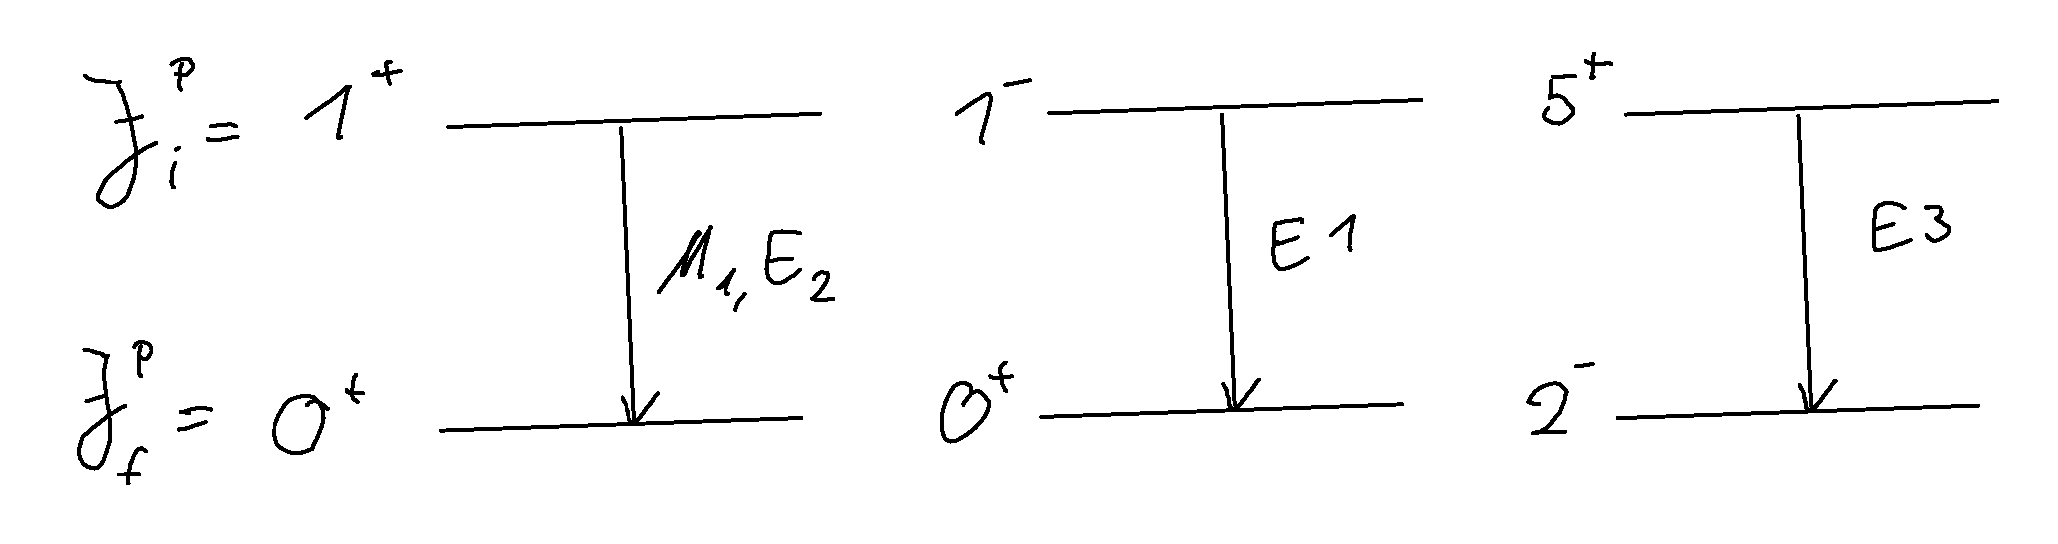
\includegraphics[width=.5\textwidth]{imgs/ep5-fig-5-14.pdf}
\caption{Häufig: Kaskaden über Zwischenzustände\label{fig:5.14}}
\end{figure}\\
\tb{Typische Lebensdauern}\\
$10^{-15} \dots 10^{-9}$\,s\\
Aber: Übergänge mit $\labs \Delta J \rabs \geq 4$ können längerlebig sein, z.B. 
\begin{align*}
^{110}Ag^\star (6^+) \overset{M4}{\ra}\ ^{110}Ag(2^-) + \gamma
\end{align*}
mit $T_{\nicefrac{1}{2}} = 235$\,d (\glqq Isomere\grqq)\\
\tb{Bemerkung:} $6^+$ entspricht $J=6$ und positiver Parität
\item \tb{Innere Konversion}\\
Alternativ zu $\gamma$-Emission
\begin{align}
\boxed{\left( ^A_Z X^\star_N \right)^0 \ra \left( ^A_Z X_N \right)^+ + e^-}
\end{align}
nachfolgend Röntgenstrahlung oder Auger-Elektron
\end{itemize}


\section{Kernspaltung}
Aufbrechen eines Kerns in zwei Tochterkerne und Neutronen:
\begin{align*}
\boxed{^A_ZX_N \ra ^{A_1}_{Z_1}{Y_1}_{N_1} + ^{A_2}_{Z_2}{Y_2}_{N_2} + kn}\\
A = A_1 + A_2 + k; \ Z = Z_1 + Z_2; \ N = N_1 + N_2 +k
\end{align*}
$Q$-Wert $>$ 0 für schwere Kerne, aber: Coulomb-Barriere\\
Kernspaltung kann (in Bezugnahme zum Tröpfchenmodell) beschrieben werden als Verformung:

\begin{figure}[!ht]
	\centering
	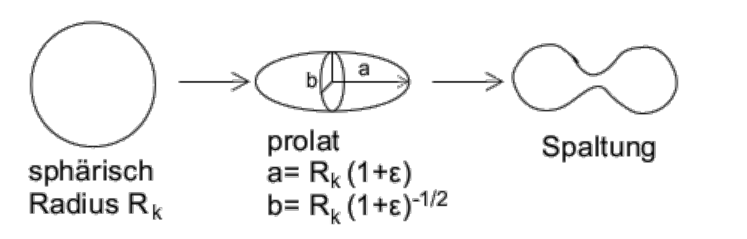
\includegraphics[width=.6\textwidth]{imgs/ep5-fig-5-15.pdf}
	\caption{Verzerrung des \glqq Nukleonentropfens\grqq{} bis hin zur Spaltung in zwei neue \glqq Tropfen\grqq \label{fig:5.15}}
	\end{figure}

\begin{figure}[!ht]
	\centering
	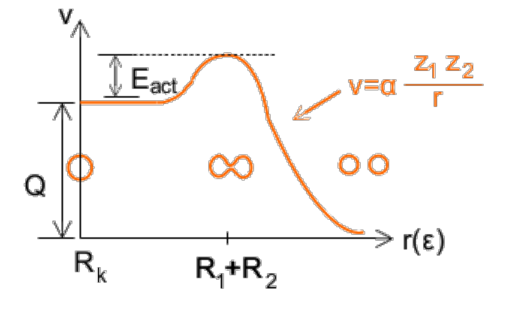
\includegraphics[width=.5\textwidth]{imgs/ep5-fig-5-16.pdf}
	\caption{Schematische Skizze zur Aktivierungsenergie $E_\mr{act}$, die für eine Kernspaltug nötig ist \label{fig:5.16}}
\end{figure}

\tb{3 Fälle:}
\begin{itemize}
\item[(i)] $E_\mr{act} < 0$ $\Ra$ Kern nicht gebunden
\item[(ii)] $E_\mr{act} > 0$, aber klein\\\
$\Ra$ Spontane Spaltung durch Tunnelprozess (ähnlich $\alpha$-Zerfall)
\item[(iii)] $E_\mr{act} > 0$ und groß\\
$\Ra$ Spaltung erfordert Energiezufuhr
\end{itemize}
\tb{Im Tröpfchenmodell:}
$E_s$, $E_c$ hängen von $\epsi$ ab.
\begin{align*}
\lno \begin{matrix}
E_s (\epsi) = a_s A^{\nicefrac{2}{3}} \left( 1+ \frac{2}{5}\epsi^2 + \dots \right) \\ E_c(\epsi) = \underbrace{a_c Z^2 A^{-\nicefrac{1}{3}}}_\text{Weizsäcker-Formel} \left( 1 - \frac{1}{5} \epsi^2 + \dots \right)
\end{matrix} \rrb \text{ohne Rechnung (Taylorentwicklung)}\\
\Ra \Delta E (\epsi) =\lno M(A,Z) \rabs_\epsi - \lno M(A,Z) \rabs_{\epsi=0} = \frac{\epsi^2}{5} \left( 2 a_s A^{\nicefrac{2}{3}} - a_c Z^2 A^{-\nicefrac{1}{3}}\right)
\end{align*}
\begin{itemize}
\item[$\Ra$] \tb{Fall (i)}, wenn $\Delta E (\epsi) < 0$
\begin{align}
\lt \ \boxed{\frac{Z^2}{A} > \frac{2 a_s}{a_c} \approx 48}
\end{align}
\begin{itemize}
\item[$\lt$] erfüllt für $Z \geq 114$, $A \gtrsim 290$
\item[$\lt$] Solche Kerne sind nicht gebunden $\ra$ nicht existent
\end{itemize}
\tb{Fall (ii): Spontane Spaltung}
\begin{align}
\begin{matrix}
 & \nearrow & ^{234}_{90}\mr{Th} & \left(\sim 100 \%\right) \qquad \text{Zerfall}\\
^{238}_{92} \mr U & & & \\
 & \searrow & \dots & \left(5\cdot 10^{-5}\%\right) \qquad \text{Spaltung}
\end{matrix}
\end{align}
\tb{Fall (iii): Induzierte Spaltung}\\
Insbesondere durch Beschuss mit Neutronen.\\
Beispiel:
\begin{align*}
^{238}_{92} \mr U + n \ra ^{239}_{92} \mr U + E_\mr{exc}
\end{align*}
Energiebilanz:
\begin{align}
\boxed{E_\mr{exc} = \underbrace{M(A,Z) + M_n - M(A+1, Z)}_{\Delta M (A,Z)} + T_n}\\
 T_n \ = \ \text{kin. Energie des Neutrons}\nonumber
\end{align}
Spaltung, falls $E_\mr{exc} > E_\mr{act}$\\
$\Ra$ 2 Fälle
\begin{itemize}
\item[(i)] $\Delta M (A,Z) > E_\mr{act}$: $T_n$ wird \glqq nicht benötigt\grqq{}, Spaltung durch langsame Neutronen\\
z.B. $^{235}_{92}\mr U$, $^{233}_{90}\mr{Th}$, $^{239}_{94} \mr{Pu}$
\begin{compactitem}
\item[$\lt$] Kettenreaktion
\item[$\lt$] gu-Kern + n $\ra$ gg-Kern
\end{compactitem}
\item[(ii)] $\Delta M(A,Z) < E_\mr{act}$ $\Ra$ $T_n \geq E_\mr{act} - \Delta M(A,Z)$\\
$\Ra$ Spaltung durch schnelle Neutronen. Z.B.:
\begin{align*}
^{238}_{92}\mr U \ \left( T_n \gtrsim 0.6\,\mr{MeV}\right)
\end{align*}
\end{itemize}
\tb{WQ für n-Einfang} (vgl. Kap.\ref{chap:3})
\begin{align}
\boxed{\sigma_n \sim \frac{1}{j_n} \sim \frac{1}{v_n} \sim \frac{1}{\sqrt{T_n}}}
\end{align}
$\Ra$ n-Einfang \tb{viel} effizienter für thermische als für schnelle Neutronen
\end{itemize}
\section{Das Prinzip von Kernreaktoren}
Kettenreaktion durch n-Einfang
\begin{align*}
^{235}_{92}U + n \ra X + Y + \lla 2.5 n\rra
\end{align*}
\tb{Multiplikationsfaktor}
\begin{align*}
\boxed{k = \frac{\# \text{sekundäre Spaltungen}}{\text{Primärspaltung}}}
\end{align*}
$k<1$: keine Kettenreaktionen (subkritisch)\\
$k=1$: stabile Kettenreaktion (kritisch) $\ra$ KKW\\
$k>1$: exponentielles Wachstum (superkritisch) $\ra$ Kernwaffen\\
Ein Reator muss also auf $k=1$ geregelt werden. Dies erfordert:
\begin{compactitem}
\item[$\ra$] Angereichertes $^{235}_{92}U$
\item[$\ra$] Abbremsen der n
\begin{compactitem}
\item[$\ra$] Stöße mit leichten Kernen (z.B.: $H_2O$, $D_2O$, $C$), genannt \glqq Moderator\grqq{}
\item[$\ra$] Ziel: $\frac{\Pa k}{\Pa T} < 0$
\begin{compactitem}
\item[$\lt$] Stabilisierend, z.B. für $H_2O$, $D_2O$
\end{compactitem}
\end{compactitem}
\item[$\ra$] Regelung der n-Dichte
\begin{compactitem}
\item[$\ra$] n-Absorber (z.b. $Cd$), genannt \glqq Kontrollstäbe\grqq{}
\end{compactitem}
\end{compactitem}
\begin{figure}[!ht]
\centering
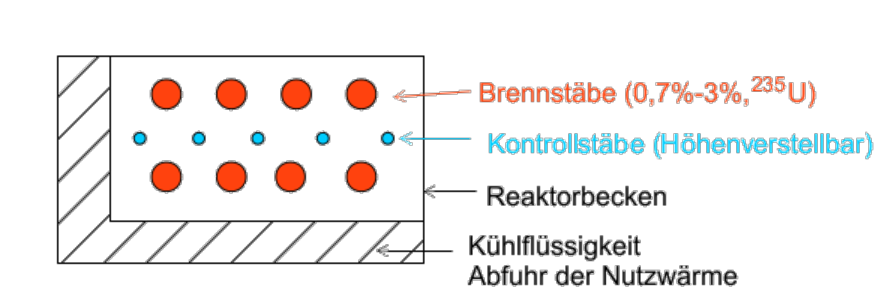
\includegraphics[width=.6\textwidth]{imgs/ep5-fig-5-17.pdf}
\caption{Schematischer Aufbau eines Reaktorbeckens \label{fig:5.17}}
\end{figure}
Nach Abschaltung:
\begin{compactitem}
\item keine Kettenreaktion
\item Aber \glqq Nachzerfallswärme\grqq{} durch radioaktive Zerfälle und Restneutronen
\item[$\ra$] unkontrollierter Anstieg der Temperatur, wenn das Kühlsystem versagt (\glqq Kernschmelze\grqq{}, z.B. Tschernobyl und Fukushima)
\end{compactitem}
